\documentclass{beamer}
\usepackage[english,russian]{babel}
\usepackage[cp1251]{inputenc}
\usepackage{caption}
\graphicspath{{fig/}}
\usepackage{amssymb}
\usepackage{enumitem}
\usepackage{comment}
\usepackage{pifont}
\usepackage{setspace}
\usepackage{blindtext}
\usepackage{epstopdf}
\usepackage{graphicx}
\usepackage{subcaption}
\ifpdf\usepackage{epstopdf}\fi
\mode<presentation>
{
  \setbeamertemplate{background canvas}[vertical shading][bottom=red!10,top=blue!10]

  \usetheme{Warsaw}
  \usefonttheme[onlysmall]{structurebold}
}

\newcommand{\dotto}{\mathrel{\ooalign{\hfil$\to$\hfil\cr\hfil$\colon$\hfil\cr}}}
% отключить клавиши навигации
\def\beq{\begin{eqnarray}}
\def\eeq{\end{eqnarray}}
\def\ee{\varepsilon}
\def\lm{\lambda}
\def\ff{\Lambda}
\def\tff{\widetilde \Lambda}
\def\P{{\cal P}}
\def\mprl{\mbox{\tiny $\|$}}
\def\mprp{\mbox{\tiny $\bot$}}

\newcommand{\ii}{\mathrm{i}} 
\newcommand{\dd}{\mathrm{d}} 
\newcommand{\eee}{\mathrm{e}} 


\newcommand{\prp}[1]{#1_{\mbox{\tiny $\bot$}}}
\newcommand{\pprl}[1]{#1_{\mbox{\tiny $\|$}}}
\setbeamertemplate{navigation symbols}{}
% Стиль презентации
	\usetheme{Warsaw}
\begin{document}
	% Стиль презентации
		\title[Перенос излучения...]{Перенос излучения равновесной электронной плазмы с учетом резонансного комптоновского процесса.}  

\author{Шленев Денис Михайлович}

\date{16 июля 2026 г.} 

\institute[] 
{
	ЯВВУ ПВО имени Маршала Советского Союза Л.А.Говорова\\ 
	\medskip
	в соавторстве с Д.А. Румянцевым и А.А. Ярковым\\ ЯрГУ им. П.Г. Демидова.
	\vspace{5mm}
	
	
	\textbf{\normalsize Физика нейтронных звёзд -- 2026}
}
%\date{16 июля 2026 г.} 


	% Создание заглавной страницы
\titlepage
%%%%%%%%%%%%%%%%%%%%%%%%%%%%%%%%%%%%%%%%%%%%%%%%%%%%%%%%%%%%%%%%%%%%%%%%%%%%%%%%%%%%%%%%
\begin{frame}{Объект исследования}
\begin{center}
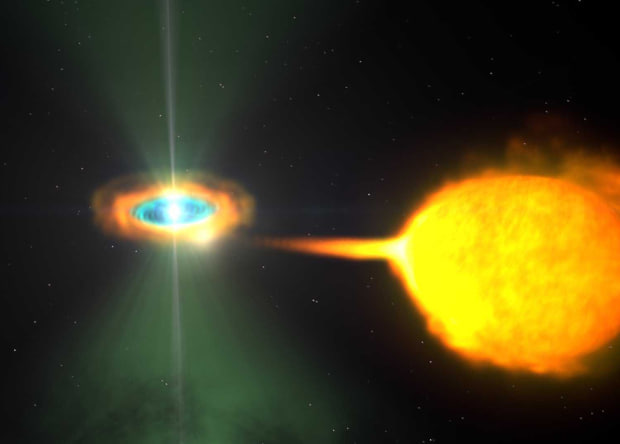
\includegraphics[width=0.9\linewidth,clip]{1.jpg}
Аккрецирующая на нейтронную звезду электронная зарядово симметричная плазма в магнитном поле порядка $\sim 10^{12}$ Гс.
\end{center}
\end{frame}
%%%%%%%%%%%%%%%%%%%%%%%%%%%%%%%%%%%%%%%%%%%%
%%%%%%%%%%%%%%%%%%%%%%%%%%%%%%%%%%%%%%%%%%%
\begin{frame}{Аккреционная колонка}\small
	\begin{columns}
		\begin{column}{0.40\linewidth}
			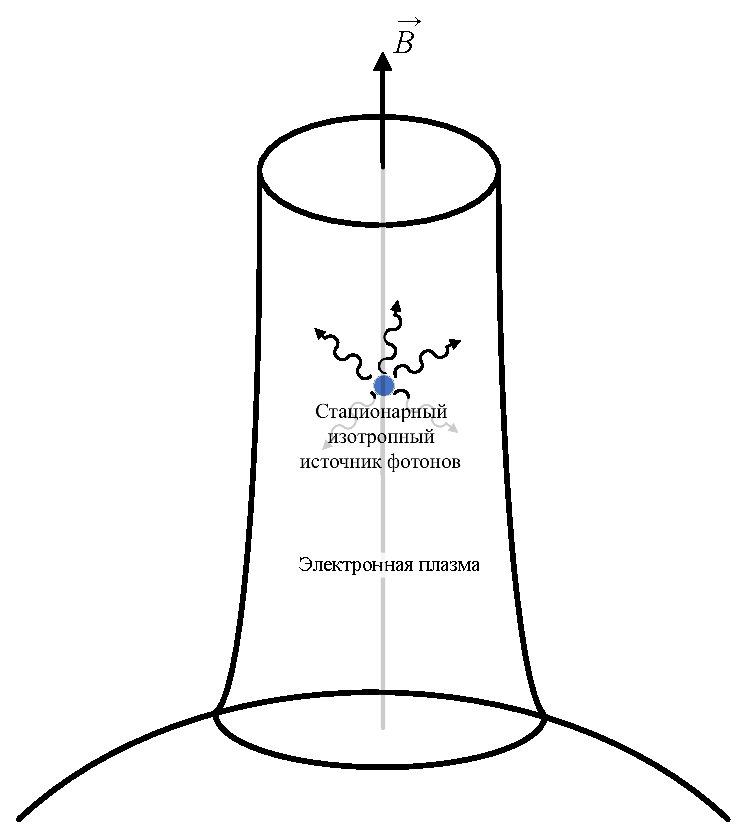
\includegraphics[width=1\linewidth,clip]{Accretion_column.eps}
		\end{column}
		\begin{column}{0.60\linewidth}
			\begin{center}
				М.М. Баско и Р.А. Сюняев 1976 -- основы теории аккреционных колонок.
				
				\vspace{3mm}
				\linespread{0.95}\selectfont
				\fontsize{9}{12}\selectfont
				В работе рассмотрена колонка зарядово-симметричной ($\mu=0$) равновесной плазмы электронов (электроны, ионы и др.) в относительно сильном поле $B\lesssim B_e$, направленном вдоль оси z. 
				
				Внутри колонки $T=\text{const}$ и $B=\text{const}$. 
				
				Через эту колонку проходит стационарный поток фотонов, испытывающих только комптоновское рассеяние. 
				
				Колонка имеет температуру $T\ll m$, поэтому электроны преимущественно занимают основной уровень Ландау. 
			\end{center}
		\end{column}
	\end{columns}
	% Справка
	% Her X-1 r0 = 44m, T_e = 6.25 10^7 К (5.39 кэВ) 
	%%%%%%%%%%%%%%%%%%%%%%%
	%LMC X-4 r0 = 680m, T_e = 5.9 10^7 К (5.08 кэВ)
	%%%%%%%%%%%%%%%%%%%%%%%%
	%Cen X-3 r0 = 730m, T_e = 3.4 10^7 К
\end{frame}

%%%%%%%%%%%%%%%%%%%%%%%%%%%%%%

\begin{frame}{Влияние замагниченной плазмы}
	\begin{center}
		Две составляющие влияния внешней активной среды:
	\end{center}
	\begin{itemize}
		\item \alert{Модификация амплитуд процессов}
		
		Становятся возможными \alert{резонансы} на виртуальном электроне.
		
		\begin{itemize}
			\item Комптоновское рассеяние $e\gamma\to e \gamma$,
			\item и др.
		\end{itemize}
		\item \alert{Модификация дисперсионных свойств частиц -- открытие новых 
		каналов:}
		Рождение пары $\gamma \to e^+e^-$\\
		Поглощение фотона $\gamma e^\pm\to e^\pm$\\
		Рождение фотона $e^\pm\to e^\pm\gamma$\\
		и др.
	\end{itemize}
\end{frame}

%%%%%%%%%%%%%%%%%%%%%%%%%%%%%%%%%%%%%%%%%%%%%%%%%%%%%%%%

\begin{frame}{\small Поляризационные свойства фотонов}
	
	\begin{center}	
		\fontsize{10pt}{12pt}\selectfont
		
		В пределе $eB\gg T^2,m^2,\omega^2$ и в зарядово симметричной плазме 
		($\mu=0$) векторы поляризации будут такими же, как и в чистом магнитном поле  
			(M.V. Chistyakov , D.A. Rumyantsev  2009):
		
		\begin{equation}\nonumber
			\varepsilon^{(1)}_\mu=\frac{(q\varphi )_\mu}{\sqrt{q^2_\perp}} ,\hspace{2mm}	\varepsilon^{(2)}_\mu=\frac{(q\tilde{\varphi})_\mu}{\sqrt{q^2_\shortparallel}}.
		\end{equation}
		
		Здесь символы 1 и 2 соответствуют: 
		\\ $\|$ и $\perp$ поляризациям в чистом магнитном поле (S.L.~Adler 1971)
		\\\fontsize{9}{11}\selectfont $X$- и $O$-  модам работы A.A. Mushtukov, D.I.~Nagirner, J.~Poutanen 2016
		\\\fontsize{9}{11}\selectfont $E$- и $O$- модам в замагниченной плазме (C.~Thompson, R.C.~Duncan 1995)
		
		\vspace{2mm}
				Возможны 4 парциальных канала рассеяния фотона:
		
		$e\gamma^{(1)}\to e\gamma^{(1)}$, $e\gamma^{(2)}\to e\gamma^{(2)}$, $e\gamma^{(2)}\to e\gamma^{(1)}$, $e\gamma^{(1)}\to e\gamma^{(2)}$. 
	\end{center}
\end{frame}



%%%%%%%%%%%%%%%%%%%%%%%%%%%%%%%%%%%%%%%%%%%%%%%%%%%%%%%%%%%%%%%%%%%%%%%%%%%%%%%%%%%%%%%%%%%%%%%%%%%%%%%%%%%%%%%%%%%	
%	\begin{frame}
%		\frametitle{Диаграммы Фейнмана}
%\begin{center}
%		Комптоновскому рассеянию отвечают две диаграммы Фейнмана:\\
%		\begin{center}{\hspace*{10mm} $s$-канал \hspace*{25mm} $t$-канал} 
%		\begin{figure}
%			\begin{center}
%				\includegraphics[width=0.6\linewidth]{CDM.jpg} 
%			\end{center} 
%		\end{figure}
%	\end{center}
%	$p^{\mu}$ и ${p'}^{\mu}$ -- импульсы начального и конечного электрона.\\
%	$q^{\mu}$ и $q^{'\mu}$ --  импульсы начального и конечного фотонов,
%	%$P^{\mu} = (p+q)^{\mu}$
%\centerline{Обозначения} 
%	
%       $(ab)_{\perp} = a_x b_x + a_y b_y$, $(ab)_{\parallel} = a_0 b_0 - a_z b_z$,
%	$(a\varphi b) = a_y b_x - a_x b_y$.
%	$\varphi_{\alpha \beta} =  F_{\alpha
%		\beta} /B$ и
%	${\tilde \varphi}_{\alpha \beta} = \frac{1}{2} \varepsilon_{\alpha \beta
%		\mu \nu} \varphi_{\mu \nu}$ -- обезразмеренный тензор поля и дуальный тензор соответственно.
%\end{center}
%
%	\end{frame}	



%%%%%%%%%%%%%%%%%%%%%%%%%%%%%%%%%%%%%%%%%%%%%%%%%%%%%%%%%%%%%%%%%%%%%%%%%%%%%%%%%%%%%%%%%%%%%%%%%%%%%%%%%%%%%%%%		
\begin{frame}{Параметры области излучения}
	%\scriptsize
	\centering
	Параметры аккреционных колонок (P.A. Becker 2012, 2022):
	\vspace{2mm}
	\begin{itemize}
		\item[1.] Магнитные поля: $B\sim 10^{11}-10^{12}$ Гс.
		\item[2.] Температура плазмы: $T_e \sim 10^6 - 10^7 $ К (0.5 -- 5 кэВ)
		\item[3.] Концентрация: $n_e \sim 10^{18} - 10^{22}$ см$^{-2}$ у основания.
		\item[4.] Радиус $44-730$ м (который также является радиусом горячей точки на поверхности звезды).
		\item[5.] Высота источника излучения в зависимости от светимости варьируется как $h_s \sim 10^3 - 10^5$ см.
		\vspace{2mm}
		
		O. Nishimura 2011:
		\item[6.] Размер области, в которых магнитное поле меняется не более чем на 5 \%, в дипольном приближении $h_{lfr}\simeq 180 - 340$ м при высотах от 1 до 10 км.
		% Около поверхности 300 м
		% 3 км от поверхности 195 м
		% 10 км от поверхности 
	\end{itemize}
\end{frame}
%%%%%%%%%%%%%%%%%%%%%%%%%%%%%%%%%%%

\begin{frame}{Методы решения задачи}
	%\framesubtitle{Постановка задачи}
	
	\scriptsize
	Непосредственное решение уравнения переноса излучения
	\begin{itemize}
		\item[-]  
		%			X-RAY PULSAR MODELS. I. ANGLE-DEPENDENT CYCLOTRON LINE FORMATION AND COMPTONIZATION 
		P. M\'esz\'aros, W. Nagel 1985 -- исследование циклотронных особенностей статической аккреционной колонки с однородными магнитным полем, концентрацией и температурой.
		\item[-]  
		%			FORMATION MECHANISM FOR BROAD AND SHALLOW PROFILES OF CYCLOTRON LINES IN ACCRETING X-RAY PULSARS 
		O. Nishimura 2003, 2005, 2008, 2011  -- моделирование спектра излучения областей формирования циклотроннных линий с учётом неоднородных магнитного поля, концентрации и температуры.
		\item[-] 
		%			THERMAL AND BULK COMPTONIZATION IN ACCRETION-POWERED X-RAY PULSARS	
		P.A. Becker 2007, 2012, 2022 -- современные аналитические модели спектра в аккрецирующих рентгеновских пульсарах с учётом как термальной комптонизации, так и в результате столкновений с быстро сжимающимся газом в аккреционном столбе (???).
		
	\end{itemize}
	Метод Монте-Карло
	\begin{itemize}		
		\item[-]
		%		CYCLOTRON LINE FEATURES FROM NEAR-CRITICAL MAGNETIC FIELDS : THE EFFECT OF OPTICAL DEPTH AND PLASMA GEOMETRY
		R.A. Araya, A.K. Harding 1999, 2000 -- одни из первых циклотронных линий (???), сформированных комптоновским рассеянием с учетом конечной ширины.
		\item[-]
		%			A model for cyclotron resonance scattering features
		G. Sch\"onherr et. al. 2007 -- построение модели циклотронных линий с помощью подхода функций Грина для любого предполагаемого источника фотонов.
		%			исследование влияния на форму спектра в области формирования циклотроннных линий для различных значений геометрии, напряженности магнитного поля, оптической толщины и температур. 
		\item[-] 
		% Statistical features of multiple Compton scattering in a strong magnetic field
		A.A. Mushtukov, S.S. Tsygankov et. al. 2021, 2022, 2023 -- разработаны модели переноса излучения в сильно замагниченной плазме с учётом циклотронного рассеяния и поляризации. Получены самосогласованные спектры и поляризационные характеристики.
	\end{itemize}
	%\end{enumerate}
\end{frame}

%%%%%%%%%%%%%%%%%%%%%%%%%%%%%%%%%%%
\begin{frame}{ \small Аналитическое определение функции распределения фотона}
	
	Кинетическое уравнение для функции распределения фотона моды $\lambda$:
	\vspace{-1mm}
	\begin{equation}\nonumber
		\hspace{-8mm}\begin{aligned}\label{Kineq:Gen}
			x\frac{\partial f^{(\lambda)}_\omega(z,x)}{\partial z}&=\sum_{\lambda'=1}^{2} \int dW_{_{e\gamma^{(\lambda)} \to e\gamma^{(\lambda')} }}\{f_{E'}(1-f_E)f^{(\lambda')}_{\omega'}(z, x') (1+f_\omega^{(\lambda)}(z, x))-
			\\
			&-f_E (1-f_{E'}) f_\omega^{(\lambda)}(z,x)(1+f_{\omega'}^{(\lambda')}(z, x'))
			\}\, .
		\end{aligned}
	\end{equation}
	
	\hspace{5mm}$x=\cos\theta$,$x'=\cos\theta'$,где $\theta$, $\theta'$ -- угол между магнитным полем и импульсом начального и конечного фотона ,$\lambda, \lambda'=1,2$ -- поляризационные состояния фотонов.
	
	\hspace{5mm}$f_\omega^{(\lambda)}, f_{\omega'}^{(\lambda')}$ -- 
	неравновесные функции распределения конечных и начальных фотонов.
	
	\hspace{5mm} $f_E=(\exp[E/T]+1)^{-1}, f_{E'}=(\exp[E'/T]+1)^{-1}$ -- равновесные функции распределения начальных и конечных электронов.
	
	\hspace{5mm}$dW_{_{e\gamma^{(\lambda)} \to e\gamma^{(\lambda')} }}$ --  дифференциальный коэффициент поглощения фотона. 
	
\end{frame}
%%%%%%%%%%%%%%%%%%%%%%%%%%%%%%%%%%%%%%%%%%%%%%%%



%%%%%%%%%%%%%%%%%%%%%%%%%%%%%%%%%%%%%%%%%
\begin{frame}
	{ \small Аналитическое определение функции распределения фотона}
	 
	Разложим кинетическое уравнение по 
	$\Delta\omega=\omega-\omega'\ll\omega$ 
	
	(А.С. Компанеец 1956, 
	Ю.Е.~Любарский~1988), где 
	\begin{equation}\nonumber
	\omega' = \frac{1}{1-x'^2}\bigg(m+\omega(1-x x')	
	- \sqrt{(m+\omega(1-x x'))^2 - 2eB (1-x'^2)}\bigg)\, .
	\end{equation}
		
		Пренебрегая индуцированным излучением, получим:
%	\begin{equation}\nonumber
%	\begin{aligned}
%	\omega' = \frac{1}{1-x'^2}\bigg(m+\omega(1-x x')-\sqrt{(m+\omega(1-x x'))^2 - 2eB (1-x'^2)}\bigg)\, ,
%	\end{aligned}
%	\end{equation}
%	где $x=\cos\theta$, $x'=\cos\theta'$. $\theta,\theta'$ - угол между импульсом фотона и магнитным полем.
	\begin{equation}\label{eq:KinSerDeltaw}\begin{aligned}\nonumber
	&\frac{\partial f^{(\lambda)}_\omega(z,x)}{\partial z} = \frac{1}{x} \sum_{\lambda'=1}^{2} \int_{-1}^{1}dx'\varphi_\omega^{\lambda\lambda'}(x,x') \bigg(f_\omega^{(\lambda')}(z,x')-f_\omega^{(\lambda)}(z,x)-
	\\
	&- \frac{\Delta \omega}{T}
	\left[
	T \frac{\partial f_\omega^{(\lambda')}(z,x')}{\partial \omega} + f_\omega^{(\lambda')}(z,x')
	\right]+
	\\
	&+ \frac{1}{2}\frac{(\Delta \omega)^2}{T^2}
	\left[
	T^2 \frac{\partial^2 f_\omega^{(\lambda')}(z,x')}{\partial \omega^2} + 2T \frac{\partial f_\omega^{(\lambda')}(z,x')}{\partial \omega}+f_\omega^{(\lambda')}(z,x')
	\right]\bigg)\, ,
	\end{aligned}
	\end{equation}
\end{frame}
%%%%%%%%%%%%%%%%%%%%%%%%%%%%%%%%%%%%%%%%%%%%%%%%%%%%%%%%%%%%%%%%%%%%%%%%%%%%%

%%%%%%%%%%%%%%%%%%%%%%%%%%%%%%%%%%%%%%%%%%%%%

\begin{frame}
	{ \small Аналитическое определение функции распределения фотона}
	
	{\fontsize{9}{11}\selectfont
	Рассматривая задачу вблизи первого ($n=1$) резонанса $\omega\simeq\omega_{res}=eB/m$, с учетом дельта-функционального приближения резонансного пика (Д.А. Румянцев и др. 2017):}
	\begin{equation}\nonumber
	\begin{aligned}
	&&\varphi^{\lambda\lambda'}_\omega(x,x') = \frac{n_e}{32 \pi m \omega} \sum_{s,s',s''=\pm 1}\int_{0}^{2\pi}\frac{d\eta}{2\pi}\times
	\\
	&&\times\frac{\left|{\cal M}^{s's''}_{e_1\to e_0\gamma^{(\lambda')}}\right|^2\left|{\cal M}^{s''s}_{e_0\gamma^{(\lambda)}\to e_1 }\right|^2}{[\omega^2(1-x^2)+2\omega m - 2eB]^2 + (\Gamma_1^{s''}P_0/2)^2}\times
	\\[2mm]
	&&\times \frac{(m+\omega - \omega x x'-\sqrt{m+\omega - \omega x x')^2 - x'^2 2eB}}{\sqrt{(m+\omega - \omega x x')^2 - x'^2 2eB}},
	\end{aligned}
	\end{equation}
	где $\Gamma_1^{s''}$ -- полная ширина поглощения электронов.
	\begin{equation}\nonumber
	E_1''\Gamma_1^{\pm} \simeq \frac{e^2 (eB)^2}{\pi M_1}\frac{1}{M_1\pm m} \int_{0}^{\zeta}dx e^{-x} \frac{1-\zeta x}{\sqrt{x^2-\zeta x+1}}
	\end{equation}
	Здесь $M_n=\sqrt{m^2+2\cdot eBn}$ и $\zeta=\frac{M_1^2+m^2}{eB}=2+B_e/B$
\end{frame}
%%%%%%%%%%%%%%%%%%%%%%%%%%%%%%%%%%%%%%%%%%%%%%%%%%%%%%%%%%%%%%%%%%%%%%%%%%%%%%	
\begin{frame}{ \small Аналитическое определение функции распределения фотона}
	
	Решение исходного уравнения в случае $f_\omega(0,x)=f_{0\omega}$ можно представить следующем образом:
	\begin{equation}\label{FormSol}\nonumber
	\begin{aligned}
	&f_\omega^{(\lambda)}(z,x)=f_{0\omega} 	e^{-{\cal \chi}_\omega^{(\lambda)}(x)\cdot z} + \frac{1}{x}\int_{0}^{z}dz'\int_{-1}^{1}dx' e^{-{\cal \chi}_\omega^{(\lambda)}(x)\cdot (z-z')}\times 
	\\
	&\times \sum_{\lambda'=1}^2\varphi_\omega^{\lambda 	\lambda'}(x,x')\bigg(f_\omega^{(\lambda')}(z,x')- \frac{\Delta \omega}{T}
	\left[
	T \frac{\partial f_\omega^{(\lambda')}(z,x')}{\partial \omega} + f_\omega^{(\lambda')}(z,x')
	\right]+
	\\
	&+ \frac{1}{2}\frac{(\Delta \omega)^2}{T^2}
	\left[
	T^2 \frac{\partial^2 f_\omega^{(\lambda')}(z,x')}{\partial \omega^2} + 2T \frac{\partial f_\omega^{(\lambda')}(z,x')}{\partial \omega}+f_\omega^{(\lambda')}(z,x')
	\right]\bigg)\, ,
	\end{aligned}	
	\end{equation}
	где $f_{0\omega}=[\exp(\omega/T)-1]^{-1}$ -- равновесная функция фотонов.
	
	\begin{equation}\nonumber
	{\cal \chi}_\omega^{(\lambda)}(x) \equiv \frac{1}{x} \int_{-1}^{1} dx' \left\{\varphi^{\lambda 1}_\omega(x,x')+\varphi^{\lambda 2}_\omega(x,x')\right\}\, .
	\end{equation}
\end{frame}

%%%%%%%%%%%%%%%%%%%%%%%%%%%%%%%%%%%%%%%%%%
\begin{frame}{ \small Аналитическое определение функции распределения фотона}
	\scriptsize
	Используя разложение функции распределения по полиномам Лежандра и выполняя преобразование Лапласа по переменной $z$, получаем:
	\begin{equation}\nonumber
		f_\omega^{(\lambda)}(z,x) = \sum_{\ell=0}^{\infty} A_\ell^{(\lambda)}(z,\omega) {\cal P}_\ell(x)\, ,
	\end{equation}
	\begin{equation}\label{eq:SysEqALap}\nonumber
		\begin{aligned}
			&\frac{2}{2 \ell +1} \overline{A}_\ell^{(\lambda)}(s,\omega) = \int_{-1}^{1} \frac{f_{0\omega}^{(\lambda)}}{s+{\cal \chi}^{(\lambda)}_\omega(x)}{\cal P}_\ell(x)dx+
			\\
			&+ \sum_{\lambda'=1}^{2}\sum_{\ell'=0}^{\infty}\frac{1}{x}\int_{-1}^{1}dx'\int_{-1}^{1}dx \frac{{\cal P}_\ell(x) {\cal P}_{\ell'}(x')}{s+{\cal \chi}_\omega^{(\lambda)}(x)} \varphi_\omega^{\lambda\lambda'}(x,x')\times
			\\
			&\times\bigg(\overline{A}_{\ell'}^{(\lambda')}(s,\omega) - \frac{\Delta \omega}{T}
			\left[
			T \frac{\partial \overline{A}_{\ell'}^{(\lambda')}(s,\omega)}{\partial \omega} + \overline{A}_{\ell'}^{(\lambda')}(s,\omega)
			\right]+
			\\
			&+ \frac{1}{2}\frac{(\Delta \omega)^2}{T^2}
			\left[
			T^2 \frac{\partial^2 \overline{A}_{\ell'}^{(\lambda')}(s,\omega)}{\partial \omega^2} + 2T \frac{\partial \overline{A}_{\ell'}^{(\lambda')}(s,\omega)}{\partial \omega}+\overline{A}_{\ell'}^{(\lambda')}(s,\omega)
			\right]\bigg)\, ,
		\end{aligned}
	\end{equation}
	где
	\begin{equation}\label{lapA}\nonumber
		\overline{A}_{\ell'}^{(\lambda)}(s,\omega)=\int_{0}^{\infty} A^{(\lambda)}_{\ell'}(z,\omega) e^{-sz}dz
	\end{equation}
\end{frame}
%%%%%%%%%%%%%%%%%%%%%%%%%%%%%%%%%%%%%%%%%%%%%%%%
\begin{frame}{ \small Аналитическое определение функции распределения фотона}
	 
	 \begin{center}
	Используя обратное преобразование Лапласа, получим функции распределения фотонов для двух возможных состояний поляризации $\lambda = 1,2$
	
	(Д.А. Румянцев, А.А. Ярков 2023):
	\end{center}
	\begin{equation}\nonumber
		\alert{	f_\omega^{(\lambda)}(z,x) = \frac{1}{2\pi i}\sum_{\ell=0}^{\infty} 
			{\cal P}_\ell(x)\int_{\sigma-i\infty}^{\sigma + i \infty}ds \cdot e^{sz} \overline{A}^{(\lambda)}_\ell(s,\omega)}
	\end{equation}
	
	
\end{frame}
%%%%%%%%%%%%%%%%%%%%%%%%%%%%%%%%%%%%%%%%
%%%%%%%%%%%%%%%%%%%%%%%%%%%%%%%%%%%%%%%%%%%%%%%%%%%%%%%%%%%%%%%%%%%%%%%%%%%%%%%%%%%%%%%%%%%%%%%%%%%%%%%%%%%%%%%%		
%\begin{frame}{Численный анализ}
%	\scriptsize
%	\centering
%	В обоих работах моделируется область циклотронных линий, а не вся аккреционная колонка целиком -- фотоны с энергиями вне резонанса практически не рассеиваются в электронной плазме, а температура, магнитное поле и концентрация можно считать постоянными.
%	\vspace{2mm}
%	\begin{columns}
		
%		\begin{column}{0.5\linewidth}
%			Работа A model for cyclotron resonance scattering features Sch\"onherr et. al. A\&A 2007.
%			\begin{itemize}
%				\item[1] Рассматривается область формирования циклотронных линий в геометрии цилиндра с бесконечной высотой и конечным радиусом с центральным расположением анизотропного источника фотонов.
%				\item[2] Задача решается с помощью моделирования Монте-Карло.
%				\item[3] Начальные фотоны задаются независимо от поляризации, т.е. спектр усреднен по поляризациям фотона.
%			\end{itemize}
%		\end{column}
%		\begin{column}{0.5\linewidth}
%			Наша работа
%			\begin{itemize}
%				\item[1] Рассматривается цилиндрическая тонкая колонка в центре которой находится анизотропный источник фотонов.
%				\item[2] Определяется функция распределения фотонов  с помощью одномерного и статического уравнения Больцмана.
%				\item[3] Решение представлено для двух возможных поляризаций фотона.
%			\end{itemize}
%		\end{column}
%	\end{columns}
%\end{frame}
%%%%%%%%%%%%%%%%%%%%%%%%%%%%%%%%%%%%%%%%%%%%%%%%%%%%%%%%%%%%%%
\begin{frame}{Численный анализ}
	\small
	Томсоновская оптическая толща в поперечном и продольном направлении:
	\begin{equation}\nonumber
		\tau_{\shortparallel T} \simeq  \sigma_T n_e z,
	\end{equation}
	\begin{equation}\nonumber
		\tau_{\perp T} \simeq  \sigma_T n_e R,
	\end{equation}
	
	Условие $\tau_\parallel >>\tau_\perp$ приводит к тому, что фотоны в основном будут покидать колонку через её стенки.
	На масштабах $\tau_\perp = 10^{-4} - 10^{-3}$ можно считать, что только резонансная область даёт вклад в модификацию спектра излучения.
	
	В пределе $n_e z \ll \lambda_K^{-2}$:
	\begin{equation}\nonumber
		f_\omega^{(\lambda)}(z,x)=f_{0\omega} 	\eee^{-{\cal \chi}_\omega^{(\lambda)}(x)\cdot z},
	\end{equation}
	где $\lambda_\text{К}$ -- комптоновская длина волны.
	
	Определяется спектр, который в случае отсутствия резонансного рассеяния:
	\begin{equation}
	\nonumber
		f_{0\omega} = A\omega^{-\alpha} \eee^{-\omega/\omega_f},
	\end{equation}
	где $A$ -- нормировочный множитель, $\alpha = 2$ -- спектральный индекс фотона,  $\omega_f = 40$ кэВ -- энергия подавления.
\end{frame}

%%%%%%%%%%%%%%%%%%%%%%%%%%%%%%%%%%%%%%%%%%%%%%%%%%%%

\begin{frame}{Анализ результатов}
	\begin{figure}\centering
		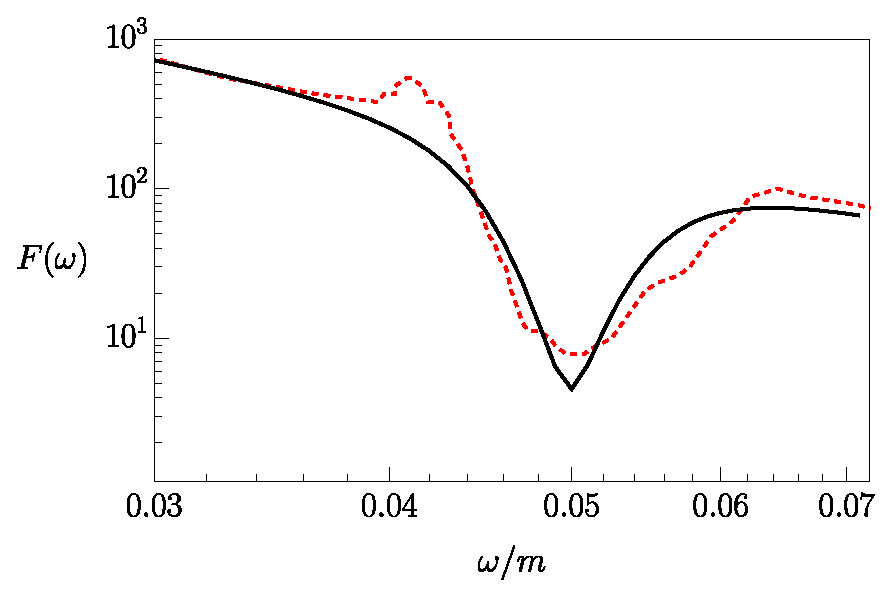
\includegraphics[width=0.8\linewidth,clip]{FDistX1tau1b005T3keVSum.eps}\hspace{1mm}
		
		\small
		Функция распределения фотона, усредненная по объему колонки, поляризации фотона (???), а также по угловому диапазону $x=cos \theta=[0.875, 1)$ при магнитном поле $B=0.05 B_e$ и температуре $T=3$ кэВ, при концентрации $n_e=10^{19} \text{ см}^{-3}$ и $z_{\text{max}} \simeq 150$ м . Штриховая линия соответствует результатам, полученным в работе Sch\"onherr et. al. A\&A 2007 для поперечной оптической толщи $\tau_T=3 \times 10^{-4}$, что соответствует радиусу колонки $R=0.45$ м.
	\end{figure}
\end{frame}
%%%%%%%%%%%%%%%%%%%%%%%%%%%%%%%%%%%%%%%%%%%%%
\begin{frame}{Анализ результатов}
	\begin{figure}\centering
		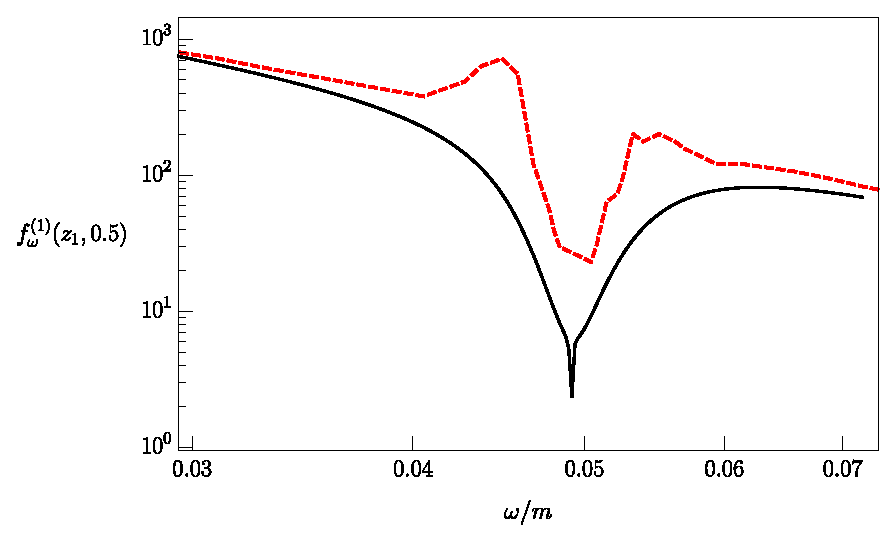
\includegraphics[width=0.8\linewidth,clip]{FDistX05tau1b005T3keVSum.eps}\hspace{1mm}
		
		\small
		Функция распределения фотона, усредненная по объему колонки, поляризации фотона, а также по угловому диапазону $x=cos \theta=[0.5, 0.625)$ при магнитном поле $B=0.05 B_e$ и температуре $T=3$ кэВ, при концентрации $n_e=10^{19} \text{ см}^{-3}$ и $z_{\text{max}} \simeq 150$ м . Штриховая линия -- Sch\"onherr et. al. 2007.
	\end{figure}
\end{frame}
%%%%%%%%%%%%%%%%%%%%%%%%%%%%%%%%%%%%%%%%%%%%%
%%%%%%%%%%%%%%%%%%%%%%%%%%%%%%%%%%%%%%%%
%%%%%%%%%%%%%%%%%%%%%%%%%%%%%%%%%%%%%%%%
%%%%%%%%%%%%%%%%%%%%%%%%%%%%%%%%%%%%%%%%%%%%%%%%%%%%%%%%%%%%%%
\begin{frame}{Анализ результатов}
	\begin{figure}\centering
		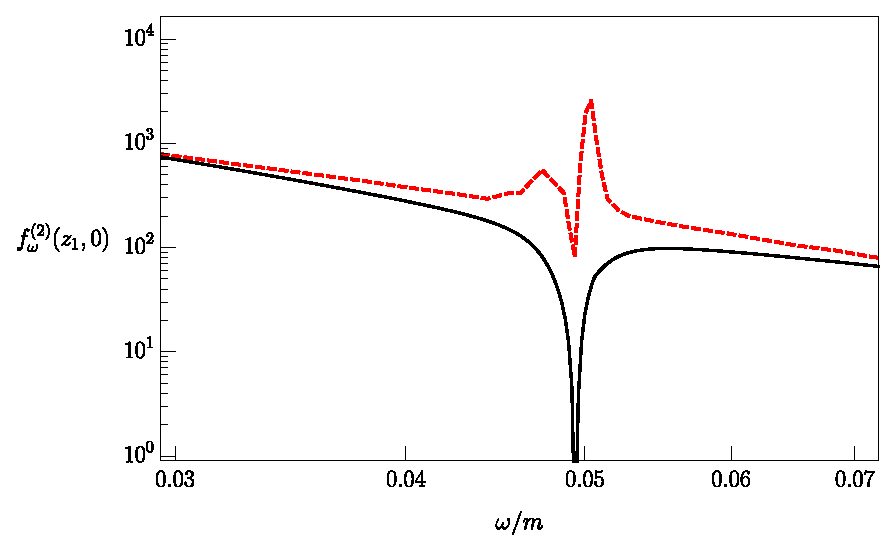
\includegraphics[width=0.8\linewidth,clip]{FDistX0tau1b005T3keVSum.eps}\hspace{1mm}
		
		\small
		Функция распределения фотона, усредненная по объему колонки, поляризации фотона (???), а также по угловому диапазону $x=cos \theta=(0, 0.125)$ при магнитном поле $B=0.05 B_e$ и температуре $T=3$ кэВ, при концентрации $n_e=10^{19} \text{ см}^{-3}$ и $z_{\text{max}} \simeq 150$ м . Штриховая линия -- Sch\"onherr et. al. 2007.
	\end{figure}
\end{frame}

%%%%%%%%%%%%%%%%%%%%%%%%%%%%%%%%%%%%%%%%%%%%%
%%%%%%%%%%%%%%%%%%%%%%%%%%%%%%%%%%%%%%%%%%%%%%%%%%%%%%%%%%%%%%%%%%%%%%%%%%%%%%%%%%%%%%%%%%%%%
%%%%%%%%%%%%%%%%%%%%%%%%%%%%%%%%%%%%%%%%%%%%

\begin{frame}	
	\frametitle{Заключение}
	\begin{itemize}[label=\textbullet]
		\item Рассмотрено решение кинетического уравнения для нахождения функции распределения фотонов двух возможных поляризаций в равновесной электронной плазме в относительно сильном магнитном поле в приближении холодной плазмы и с учётом резонанса на виртуальном электроне.
		\item С помощью преобразования Лапласа и разложения функции распределения по полиномам Лежандра задача сведена к системе дифференциальных уравнений.
		\item Представлен сравнительный анализ с результатами, полученными в литературе с помощью моделирования Монте-Карло. Показано, что результаты достаточно хорошо описывают вклад резонансного Комптона в формирование спектра излучения области циклотронных линий.
	\end{itemize}
\end{frame}
%%%%%%%%%%%%%%%%%%%%%%%%%%%
\begin{frame}{Что дальше?}
	Для улучшения сходимости результатов планируется предпринять следующее:
	\begin{itemize}
		\item[1)] Рассмотреть следующие резонансы, соответствующие уровням Ландау $n\geq 2$.
		\item[2)] Учет следующих поправок к пределу узкого резонансного пика Румянцев Д.А., Ярков А.А., Шленев Д.М., ЖЭТФ, 2026
		\item[3)] Учет конечного радиуса колонки.
	\end{itemize}
\end{frame}
%%%%%%%%%%%%%%%%%%%%%%%%%%%%%%%%%%%%%
\begin{frame}
	\begin{figure}\centering
		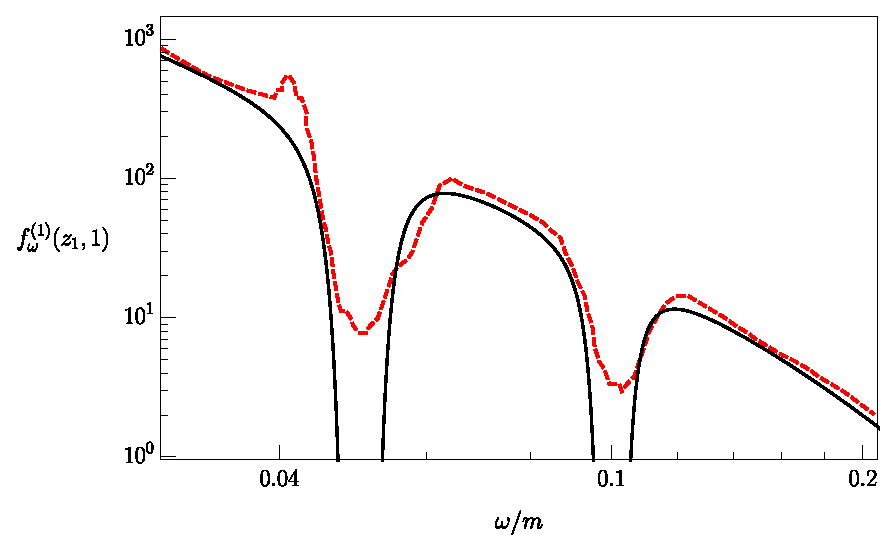
\includegraphics[width=0.49\linewidth,clip]{FDistX1tau1b005T3keVMode1.eps}\hspace{1mm}
		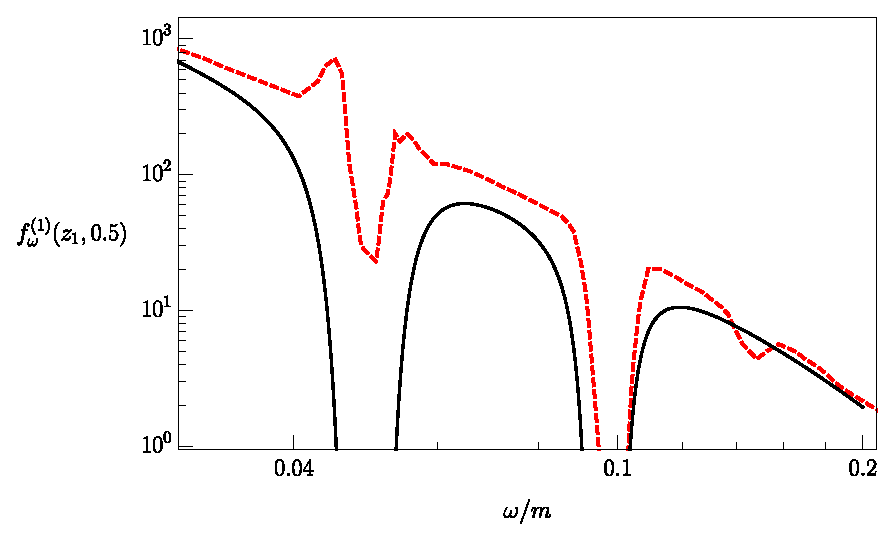
\includegraphics[width=0.49\linewidth,clip]{FDistX05tau1b005T3keVMode1.eps}\\
		
		Функция распределения фотона моды 1 при магнитном поле $B=0.05 B_e$ и температуре $T=3$ кэВ,  для углов $\theta = 0$ ($x=0$) и $\theta = \pi/3$ ($x=0.5$) между направлением импульса начального фотона и направлением магнитного поля, $\tau_{1}=~3~\times 10^{-4}$. Штриховая линия соответствует результатам, полученным в работе Schonherr:2007, сплошная линия -- дельта-функциональному приближению. Концентрация электронов -- $n_e \approx 10^{12}\text{ см}^{-3}$.
	\end{figure}
\end{frame}
%%%%%%%%%%%%%%%%%%%%%%%%%%%%%%%%%%%%%%%%%%%%%
\begin{frame}
\begin{columns}
	\begin{column}{0.49\linewidth}
		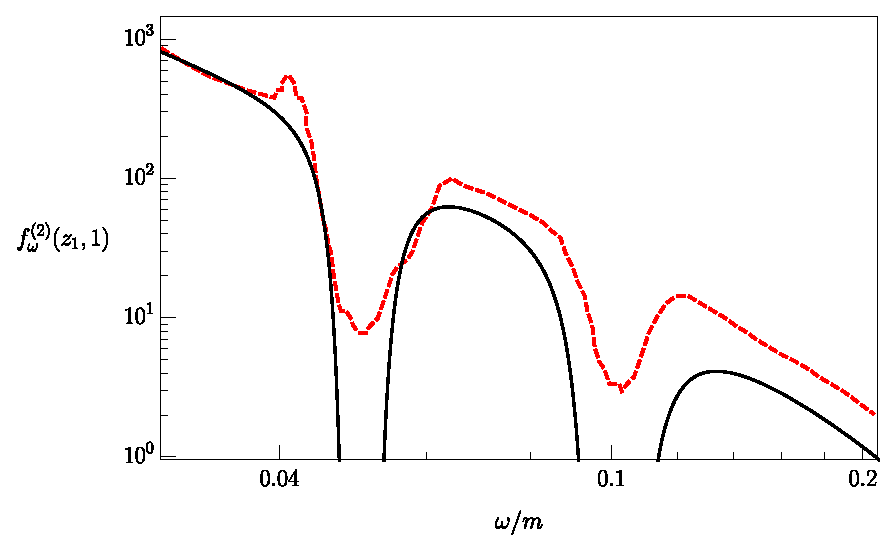
\includegraphics[width=1\linewidth,clip]{FDistX1tau1b005T3keVMode2.eps} \hspace{1mm}
		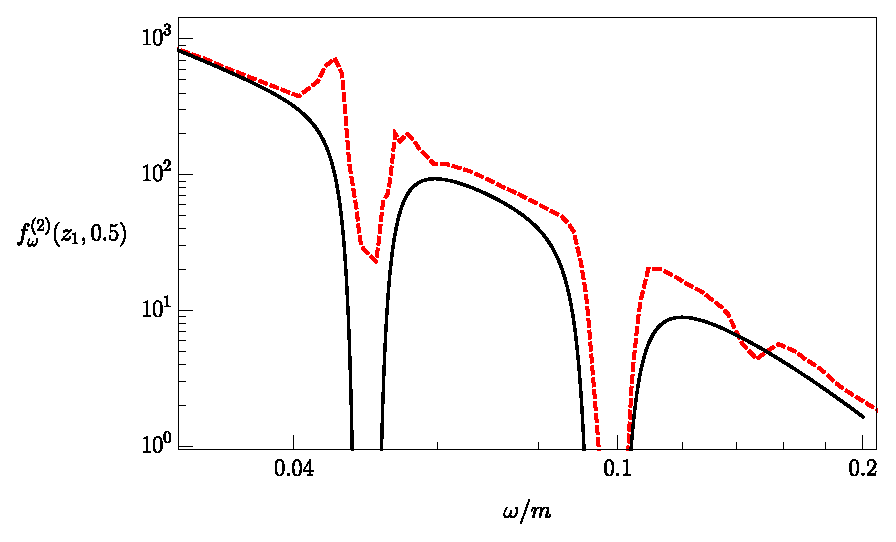
\includegraphics[width=1\linewidth,clip]{FDistX05tau1b005T3keVMode2.eps}
	\end{column}
	\begin{column}{0.55\linewidth}
			\vspace{4mm}
			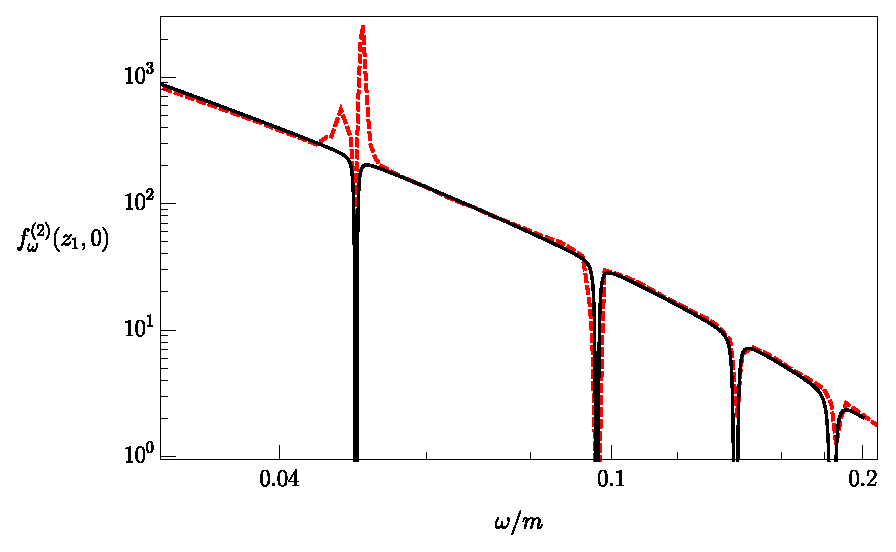
\includegraphics[width=1\linewidth,clip]{FDistX0tau1b005T3keVMode2.eps}
			\begin{center}
				\linespread{0.95}\selectfont
				\small Функция распределения фотона моды 2 при  $B=0.05 B_e$ и  $T=3$ кэВ, для углов $\theta = 0$ ($x=0$), $\theta = \pi/3$ ($x=0.5$) и $\theta=\pi/2$ ($x=1$), а также оптической толщи~$\tau_{1}=~3~\times 10^{-4}$. Штриховая линия соответствует результатам, полученным в работе Schonherr:2007, сплошная линия -- дельта-функциональному приближению. Концентрация электронов -- $n_e \approx 10^{12}\text{ см}^{-3}$.
			\end{center}
	\end{column}
\end{columns}
\centering

\end{frame}
%%%%%%%%%%%%%%%%%%%%%%%%%%%%%%%%%%%%%%%
%%%%%%%%%%%%%%%%%%%%%%%%%%%%%%%%%%%%%%%
\begin{frame} 
\begin{figure}\centering
	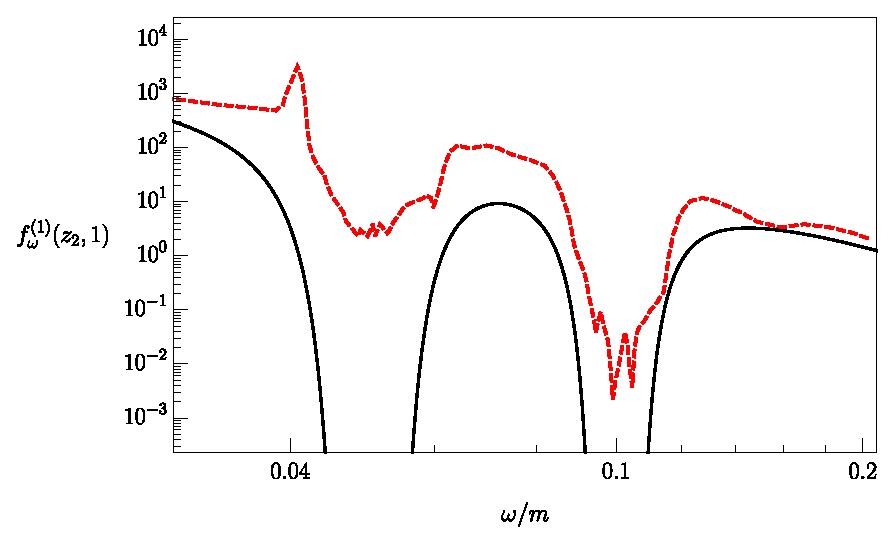
\includegraphics[width=0.49\linewidth,clip]{FDistX1tau2b005T3keVMode1.eps}\hspace{1mm}
	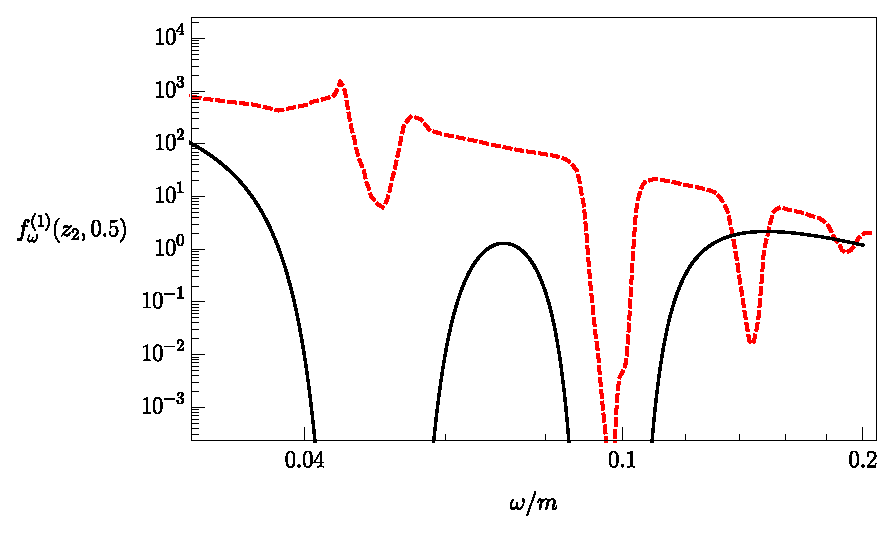
\includegraphics[width=0.49\linewidth,clip]{FDistX05tau2b005T3keVMode1.eps}\\
	Функция распределения фотона моды 1 при $B=0.05 B_e$ и $T=3$ кэВ  для углов $\theta = 0$ ($x=0$) и $\theta = \pi/3$ ($x=0.5$) между направлением импульса начального фотона и направлением магнитного поля, а также оптической толщи~$\tau_{2}=~3~\times 10^{-3}$. Штриховая линия соответствует результатам, полученным в работе Schonherr:2007, сплошная линия -- дельта-функциональному приближению. Концентрация электронов -- $n_e \approx 10^{12}\text{ см}^{-3}$.
\end{figure}
\end{frame}
%%%%%%%%%%%%%%%%%%%%%%%%%
%%%%%%%%%%%%%%%%%%%%%%%%%
\begin{frame} 
\begin{columns}
	\begin{column}{0.49\linewidth}
		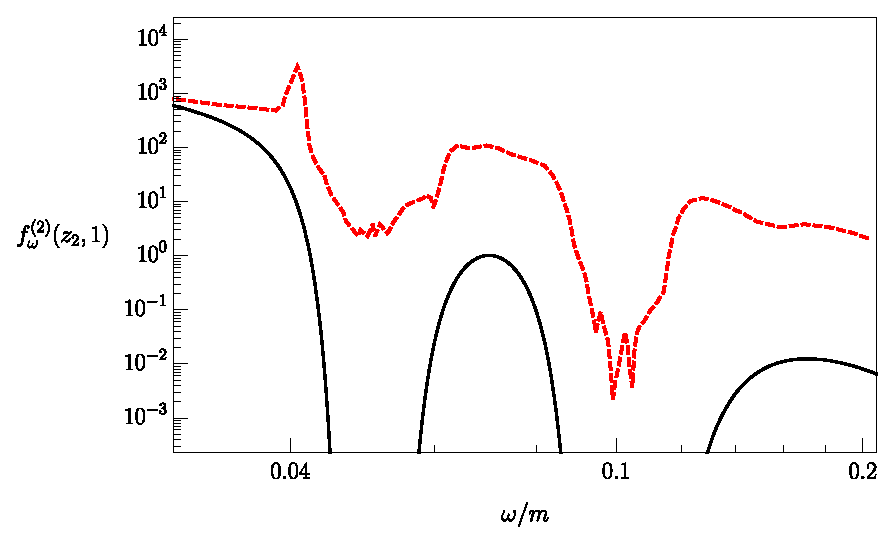
\includegraphics[width=1\linewidth,clip]{FDistX1tau2b005T3keVMode2.eps} \hspace{1mm}
		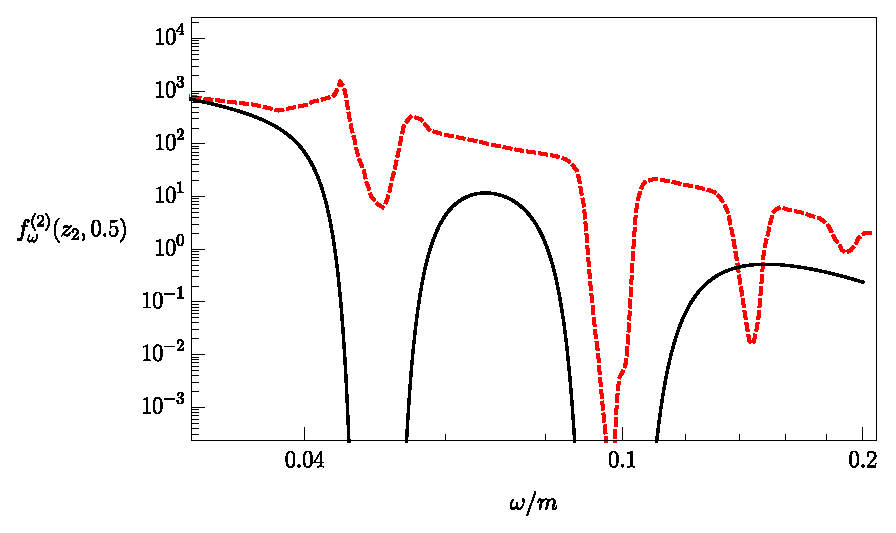
\includegraphics[width=1\linewidth,clip]{FDistX05tau2b005T3keVMode2.eps}
	\end{column}
	\begin{column}{0.55\linewidth}
		\vspace{4mm}
		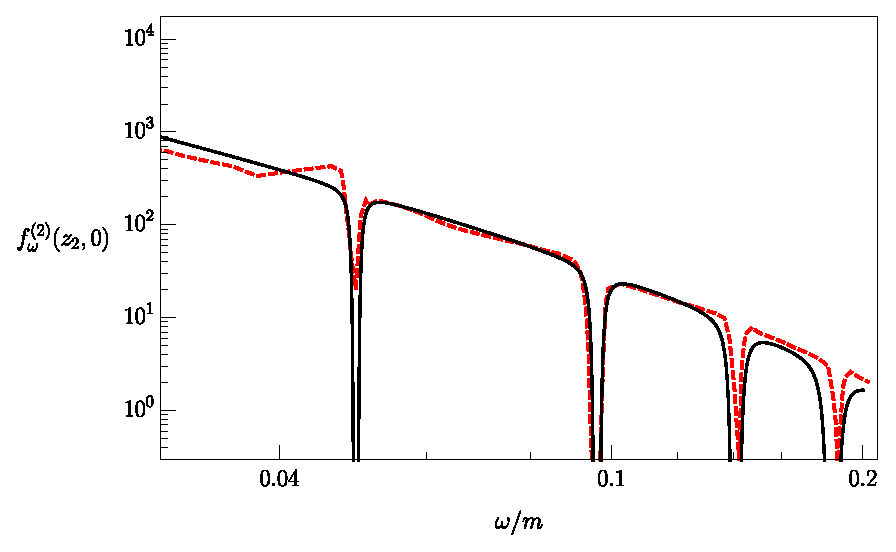
\includegraphics[width=1\linewidth,clip]{FDistX0tau2b005T3keVMode2.eps}\\
\begin{center}
	\linespread{0.95}\selectfont \small Функция распределения фотона моды 2 при $B=0.05 B_e$ и $T=3$ кэВ, для углов $\theta = 0$ ($x=0$), $\theta = \pi/3$ ($x=0.5$) и $\theta=\pi/2$ ($x=1$), а также оптической толщи~$\tau_{2}=~3~\times 10^{-3}$. Штриховая линия соответствует результатам, полученным в работе Schonherr:2007, а сплошная линия -- дельта-функциональному приближению. Концентрация электронов -- $n_e \approx 10^{12}\text{ см}^{-3}$.
\end{center}

	\end{column}
\end{columns}
\end{frame}
%%%%%%%%%%%%%%%%%%%%%%%%%%%%%%%
%%%%%%%%%%%%%%%%%%%%%%%%%%%%%%%%%%%%%%%%%%%%%
\begin{frame}
	\begin{figure}\centering
		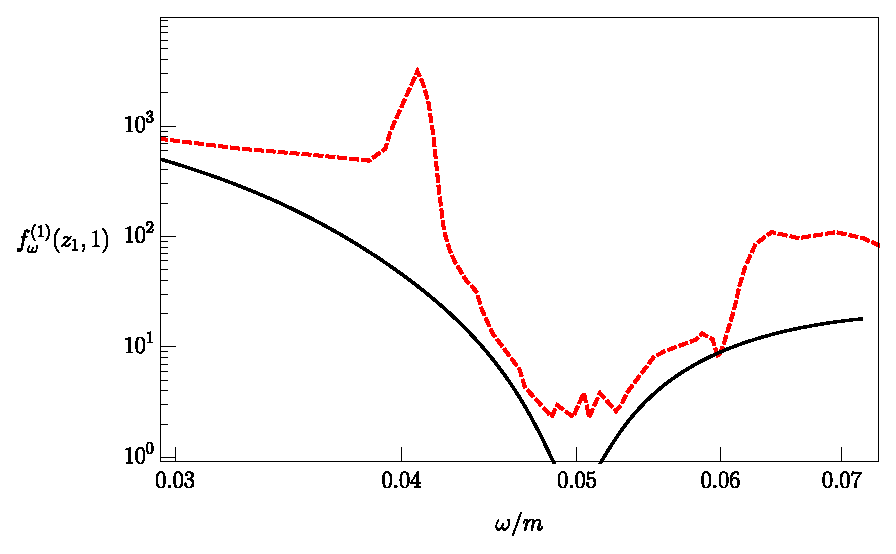
\includegraphics[width=0.8\linewidth,clip]{FDistX1tau2b005T3keVSum.eps}\hspace{1mm}
		
		Функция распределения фотона, усредненная по объему колонки, поляризации фотона, а также по угловому диапазону $x=cos \theta=[0.875, 1)$ при магнитном поле $B=0.05 B_e$ и температуре $T=3$ кэВ, $\tau_{2}=~1$, что при концентрации $n_e=10^{19} \text{ см}^{-3}$ соответствует $z_2 = z_{\text{max}} \simeq 1500$ м . Штриховая линия соответствует результатам, полученным в работе Schonherr:2007, сплошная линия -- дельта-функциональному приближению.
	\end{figure}
\end{frame}
%%%%%%%%%%%%%%%%%%%%%%%%%%%%%%%%%%%%%%%%%%%%%
\begin{frame}
	\begin{figure}\centering
		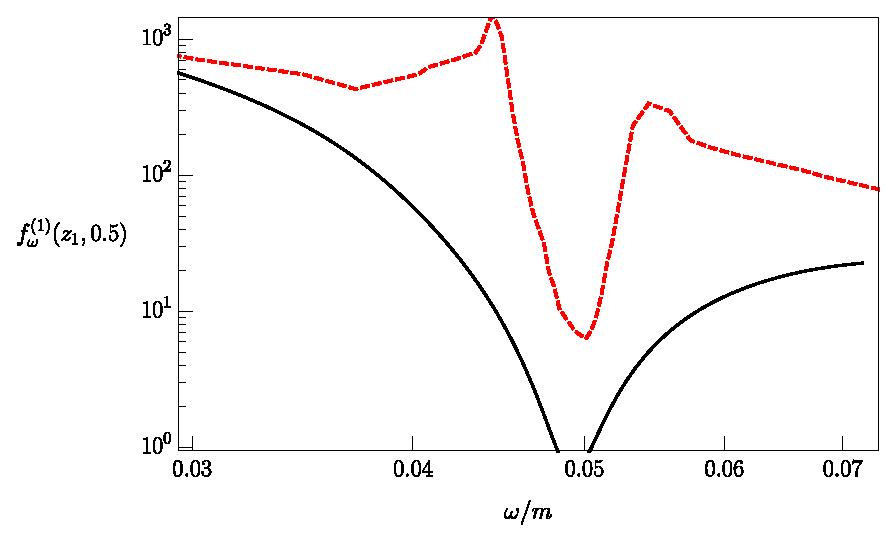
\includegraphics[width=0.8\linewidth,clip]{FDistX05tau2b005T3keVSum.eps}\hspace{1mm}
		
		Функция распределения фотона, усредненная по объему колонки, поляризации фотона, а также по угловому диапазону $x=cos \theta=[0.5, 0.625)$ при магнитном поле $B=0.05 B_e$ и температуре $T=3$ кэВ, $\tau_{2}=~1$, что при концентрации $n_e=10^{19} \text{ см}^{-3}$ соответствует $z_2 = z_{\text{max}} \simeq 1500$ м . Штриховая линия соответствует результатам, полученным в работе Schonherr:2007, сплошная линия -- дельта-функциональному приближению.
	\end{figure}
\end{frame}
%%%%%%%%%%%%%%%%%%%%%%%%%%%%%%%%%%%%%%%%%%%%%
%%%%%%%%%%%%%%%%%%%%%%%%%%%%%%%%%%%%%%%%
%%%%%%%%%%%%%%%%%%%%%%%%%%%%%%%%%%%%%%%%
%%%%%%%%%%%%%%%%%%%%%%%%%%%%%%%%%%%%%%%%%%%%%%%%%%%%%%%%%%%%%%
\begin{frame}
	\begin{figure}\centering
		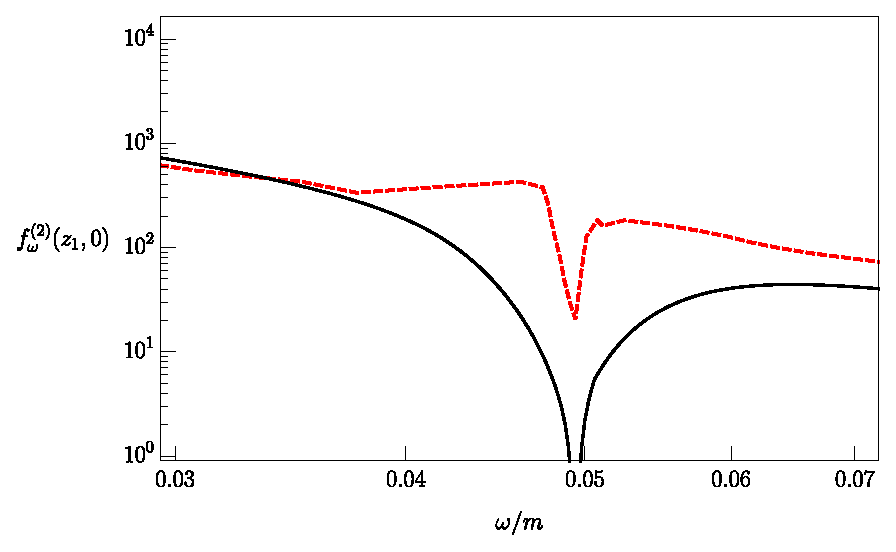
\includegraphics[width=0.8\linewidth,clip]{FDistX0tau2b005T3keVSum.eps}\hspace{1mm}
		
		Функция распределения фотона, усредненная по объему колонки, поляризации фотона, а также по угловому диапазону $x=cos \theta=(0, 0.125)$ при магнитном поле $B=0.05 B_e$ и температуре $T=3$ кэВ, $\tau_{2}=~1$, что при концентрации $n_e=10^{19} \text{ см}^{-3}$ соответствует $z_2 = z_{\text{max}} \simeq 1500$ м . Штриховая линия соответствует результатам, полученным в работе Schonherr:2007, сплошная линия -- дельта-функциональному приближению.
	\end{figure}
\end{frame}
%%%%%%%%%%%%%%%%%%%%%%%%%%%%%%%
\end{document}